\chapter{Style Extraction and Transfer}
\minitoc% Creating an actual minitoc

\par We finally arrive to the core objective of the PhD: how to leverage information of style from one (or more) tasks, in order to bootstrap the learning of a new task.

\section{Introduction and objectives}
\setlist{nolistsep}\begin{itemize}[noitemsep]
    \item Motivate transfer learning in general (general talking)
    \item Why extracting style?: on our side, as ML practitioners, the ultimate objective of using ML is to help us extract new knowledge
    \item The questions of research here: extracting styles from bottleneck, transfer between writers, transfer between tasks
\end{itemize}

\section{Transfer learning}\label{sec:transfer_learning}
\par An important research direction in machine learning nowadays is transfer learning. If humans and machines are able to learn how to perform a task, one of the thing that separates humans from machines is the ability to leverage this knowledge in order to acquire new skills and perform new tasks, without the need for additional trials and errors from tabula rasa. For example:
\setlist{nolistsep}\begin{itemize}[noitemsep]
    \item If you know how to hold a glass cup, with little adjustments, you can learn how to hold a plastic bottle.
    \item If you know probability and algebra, it will accelerate your progress in machine learning.
\end{itemize}
This however, is not a straightforward thing for machine learning to do. The algorithms are fitted to data responding directly to the task required (i.e., has the same input feature space and same distribution). Thus, a change in the task can lead to degradation in the algorithm performance \citep{shimodaira2000improving,weiss2016survey}.

\par In the following subsections, I first introduced notations and clear description for the objective of transfer learning, and the metrics used to evaluate the quality of transfer. I then discuss different types of transfer learning, with examples on each type.

\subsection{Notation and problem definition}
\par BASIC NOTATION:
\setlist{nolistsep}\begin{itemize}[noitemsep]
    \item A domain $\mathcal{D}$ is defined as $\mathcal{D} = \{\mathcal{X}, P(X)\}$, where:\\
    $\mathcal{X}$ is the feature space, $X$ is the learning sample, $X = \{x_1,x_2,\cdots,x_n\} \in \mathcal{X}$, $n$ is the size of the learning sample, $P(X)$ is the marginal distribution probability of the learning sample.

    \item For a given domain, a task $\mathcal{T}$ is defined as $\mathcal{T} = \{\mathcal{Y}, f(.)\}$, where:\\
    $\mathcal{Y}$ is the label space, $f(.)$ is the predictive function (takes $x_i$ and outputs $y_i$). It can also be rewritten as $\mathcal{T} = \{\mathcal{Y}, P(Y|X)\}$.

    \item Source domain data set, $D_S = \{(x_{1S},y_{1S}),\cdots,(x_{nS},y_{nS})\} = \{X_S,Y_S\}$.\\ Target domain data set, $D_T = \{(x_{1T},y_{1T}),\cdots,(x_{nT},y_{nT})\}= \{X_T,Y_T\}$.\\
    Source task $\mathcal{T}_s$, target task $\mathcal{T}_t$.
\end{itemize}

\GB{be careful, it's not clean!}

\par DEFINITION OF TRANSFER LEARNING: Given source domain data $D_S$, source task, $\mathcal{T}_S$,  target domain $D_T$ and target task $\mathcal{T}_T$, we wish to improve the the prediction function of the target task $f_T(.)$ by using $D_S$ and $\mathcal{T}_S$. Conditions of transfer learning are:

\setlist{nolistsep}\begin{itemize}[noitemsep]
    \item $D_S \neq D_T$, which means $\mathcal{X}_S \neq \mathcal{X}_T$ and/or $P(X_S) \neq P(X_T)$ (frequency feature bias).\\
    If $\mathcal{X}_S \neq \mathcal{X}_T$, the transfer learning problem is \textit{Heterogeneous}. Otherwise, it is \textit{Homogeneous}.

    \item $\mathcal{T}_S \neq \mathcal{T}_T$, which means $\mathcal{Y_S} \neq \mathcal{Y_T}$ and/or $P(Y_S|X_S) \neq P(Y_T|X_T)$ (context feature bias).
\end{itemize}

\paragraph{Symmetric and Asymmetric transfer} \textit{Symmetric} feature transformation attempts to discover underlying meaningful structure between domains, to find common latent features that unify (or at least reduce) the marginal distribution of the two domains. \textit{Asymmetric} feature transformation attempts to transfer the features of the source space to make them more closely match the target space. See figure \ref{fig:feature_transformation}.

\begin{figure}[!htbp]
\centering
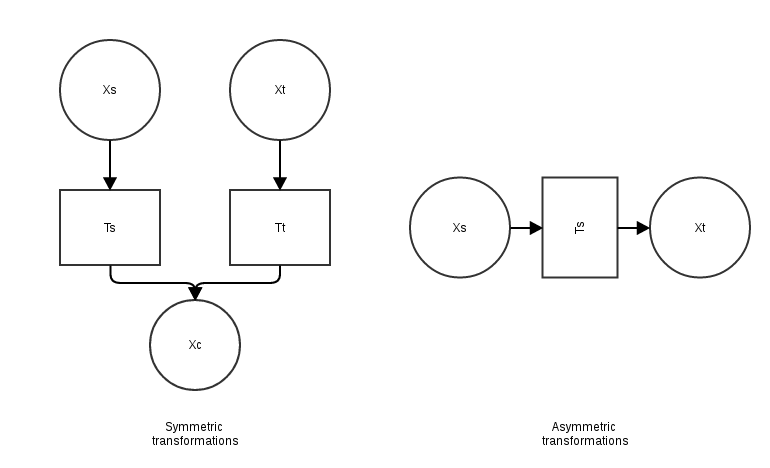
\includegraphics[scale=0.4]{images/sota/feature_transformation.png}
\caption[Symmetric and Asymmetric transfer]{Illustration for the difference between Symmetric and Asymmetric feature transformation \textbf{REDO THE DIAGRAMS -- NOT CLEAR}}
\label{fig:feature_transformation}
\end{figure}

% TODO: Complete this from the TL in RL paper
\subsection{Metrics to evaluate transfer learning}
\par There is no standard way to evaluate transfer learning. Several metrics have been proposed in the literature \citep{taylor2007cross}, like (see also figure \ref{fig:tl_metrics}) \GB{complete figure to have these 4 features}:
\begin{enumerate}
    \item Jump start: It is the difference in the initial performance between using transfer relative to learning without transfer.
    \item Asymptotic performance: The difference in the learning performance through time/epochs between using transfer relative to learning without transfer.
    \item Total Reward/Accuracy difference between end-performance with vs. without transfer learning.
    \item Time-to-threshold: It the amount of time (or number of samples) needed to achieve a pre-specific performance level.
\end{enumerate}

\begin{figure}[!htbp]
\centering
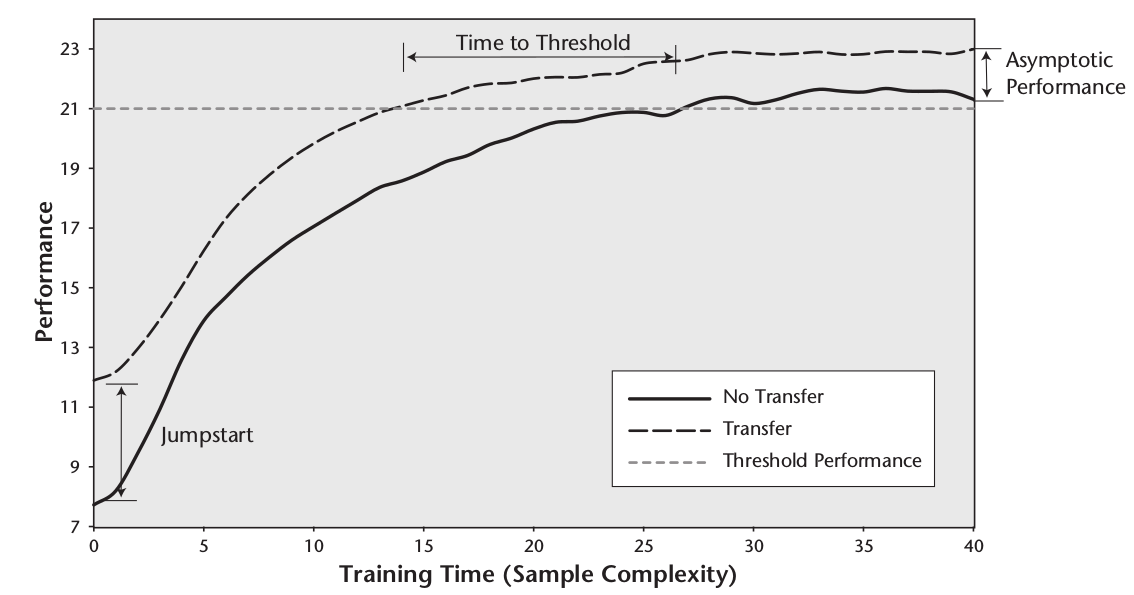
\includegraphics[scale=0.3]{images/sota/TL_metrics.png}
\caption{Different proposed metrics to measure transfer learning \textbf{Mention the source of this image}}
\label{fig:tl_metrics}
\end{figure}

\par The transfer is considered as successful if metric 1 is greater than zero, metrics 2-3 increases with transfer or metric 4 reduces through transfer. It is worth mentioning that, in most state of the art, only metrics 3 and/or \GB{4??} are reported (which are the relevant metrics in my opinion for our work). I report all those metrics however, since I believe they give us a good diagnostics for our transfer learning system.

%\section{Discussion about the state of the a}
\subsection{Homogeneous transfer learning}
\par In this case, most of the research are focused on one of the 3 areas:
\setlist{nolistsep}\begin{itemize}[noitemsep]
    \item Correct for source marginal distribution $P(X_S)$,
    \item Correct for the source conditional distribution $P(Y_S|X_S)$,
    \item Both.
\end{itemize}

\subsubsection{Symmetric - transfer learning using deep learning}
\textbf{NEEDS TO BE UPDATED}\citep{glorot2011domain} discusses a deep learning approach for transfer learning, by using using stacked de-noising auto-encoders, to correct the marginal distribution between the source and the target domain, by learning latent variables/features common between the two data sources in two steps:
\setlist{nolistsep}\begin{itemize}[noitemsep]
    \item First, train an auto-encoder on the unlabeled data from the source and the target. This will produce latent variables.
    \item Use those latent features to train a classifier on the labeled source data.
\end{itemize}
\par Experiments are done on sentimental analysis, for 12 different sources and target domain pairs. The data used reviews for different products (4 different products). \GB{Give performance}

\par The idea of using deep learning~\citep{lecun2015deep} in order to achieve transfer learning has gain popularity during the last years, following the achievements in having better computational resources~\citep{raina2009large}, and the availability of large benchmark datasets - most notably: ImageNet~\citep{imagenet_cvpr09} for object detection, MS-COCO~\citep{2014arXiv1405.0312L} for image captioning~\ldots
\GB{Give general/key idea rapidly: pre-training of feature extractions performed by layers close to input, vs. training of high-level processing performed by layers close to output.}

\par The first notable success of deep learning happened in the area of computer vision, with the AlexNet architecture~\citep{krizhevsky2012imagenet}. It was found out that such a deep network manages to extract generic features about the images: it learns simple, hierarchical filters, that are generic enough to be applicable for different datasets (see figure~\ref{fig:AlexNet_filters}). This observation led to another surge in the usage of pretrained AlexNet - and later newer architectures, like VGG16~\citep{simonyan2014very}, Inception~\citep{szegedy2015going},etc - as feature extractors for new, unseen datasets.

\begin{figure}[!htbp]
\centering
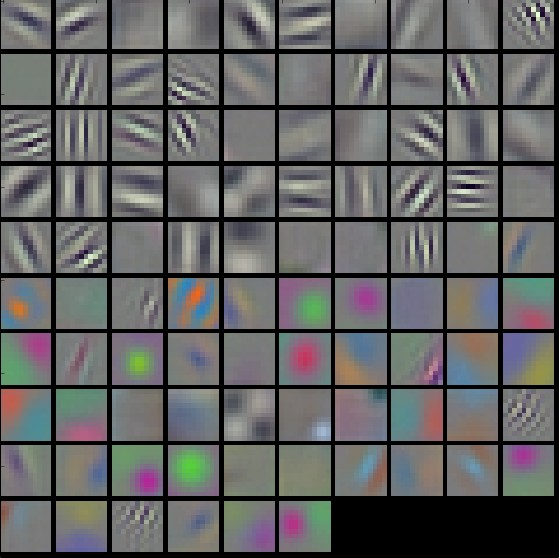
\includegraphics[scale=0.4]{images/sota/filt1.jpeg}
% \caption{Visualization of the first convolution layer of a trained AlexNet. The weights are very nice and smooth, indicating nicely converged network. Note also the basic simple shape of filters. It easy to imagine that those same filters will be useful in other computer vision or image related tasks.}
\caption[Convolution Neural Networks filters shape]{Visualization of the first convolution layer of a trained AlexNet. Note the basic shape of filters that resemble to Gabor filters widely used in image processing for decades~\citep{fogel1989gabor,jain1991unsupervised}. It easy to imagine that those same filters will be useful in other computer vision or image-related tasks.}
\label{fig:AlexNet_filters}
\end{figure}

\par It is interesting to note that those filters can be also seen as a representation for the skills we want to extract. In our case, we will need to combine both deep convolution network with a recurrent neural network (like in \citep{s16010115,pinheiro2014recurrent,huang2016deep}).

% \par Although very interesting, a major concern with this approach - as mentioned in my thesis committee report - is that almost all the studies reported\endnote{To the best of my knowledge} starts from the fact that they have large datasets. I am not aware of a study trying to build lower-boundaries for the minimal amount of data needed to have a good enough filters suitable for transfer learning.

% \subsection{Asymmetric}

\subsubsection{Parameter-based transfer}
\citep{chattopadhyay2012multisource} propose a Conditional probability based domain adaptation (CP-MDA): it corrects the difference between conditional probability distributions of multiple labeled source data, vs. limited amount of labeled target data. The process has five main steps:
\begin{enumerate}
    \item Build a classifier for each of the source domains
    \item Measure the closeness of each of those classifiers to the conditional distribution of the target domain.
%(NOTE: I don't understand yet how it is done).
    \item Weight the classifiers according to their closeness
    \item Use the weighted source classifiers to find pseudo labels for the unlabeled target data
    \item Train a new classifier to map between the pseudo labels and the real labels on the targets data
\end{enumerate}
Experiments are done on fatigue classification (surface electromyography data). Different source domain is for different people.

\subsubsection{Instance-based transfer}
\citep{chattopadhyay2012multisource} developed a weighting framework for multi-source domain adaptation (2SW-MDA). It tries to correct both the marginal and the conditional distributions between the source and the target domains in three steps:
\begin{enumerate}
    \item Weight each source domain based on the marginal distribution difference between it and the target domain
    \item Source domain weights are updated according to the (CP-MDA) approach
    \item The target classifier is learned based on the re-weighted source classifiers and the labelled target data.
\end{enumerate}
%(NOTE: To be review again how this learning happens)
Experiments are done on fatigue classification (surface electromyography data). Different source domain is for different people.

% \subsection{Relational based transfer}
% \subsection{Hybrid based transfer}

\subsection{Heterogeneous transfer learning}
\par In this case, most of the research are focused on only one area: Aligning $\mathcal{X_S}$ with $\mathcal{X_T}$, assuming that $P(X_S) = P(X_T)$.

\subsubsection{Symmetric}
\citep{shi2010transfer} developed a method called \emph{Heterogeneous Spectral Mapping} (HeMap). It is assumed that: $\mathcal{X_S} \neq \mathcal{X_T}$, $P(X_S) \neq P(X_T)$ and $\mathcal{Y_S} \neq \mathcal{Y_T}$. It also assumes the availability of labeled source data, and limited labeled target data.
\setlist{nolistsep}\begin{itemize}[noitemsep]
    \item First is to find common latent variables between the source and the target domains, by using spectral mapping techniques. The spectral mapping objective is to maintain the original data structure, while minimizing the difference between the two domains (NOTE: Review the way it is formalized).
    \item Second, a cluster based sampling is performed to selected new training data (Thus, correcting the difference in marginal distribution).
    \item Third, correct the conditional distribution by Bayesian methods (NOTE: To be reviewed again, not clear to me).
\end{itemize}
Experiments are performed on image classification and drug efficacy prediction. (NOTE: The results are not clear, as they don't mention what is the baseline exactly, and no comparison to other state of the art methods is performed).

\subsubsection{Asymmetric}
\citep{Nam:2015:HDP:2786805.2786814} discuss the application of transfer learning in software module defect problem. The source and the target software projects collect different performance metrics. The solution developed is called heterogeneous defect prediction (HDP). \endnote{This solution performs well on the assumption that the source and the target features are statistically close}.
\setlist{nolistsep}\begin{itemize}[noitemsep]
    \item First, perform feature selection on the source and on the target data, in reduce the dimensionality.
    \item Second, a statistical comparison (Kolmogorov-Smirnov test) is performed between the reduced source and target features, in order to determine the closeness of different features.
    \item Third, train a classifier using those close source features.
    \item Fourth, use this classifier on the target data, where the input will be the corresponding target features (related to the source features from the previous step).
\end{itemize}

\subsection{Negative transfer}
\par A concern that arises in transfer learning is what is called \textit{negative transfer}, where the knowledge learned from one task leads to no improvement on the target task, but reduces the quality of learning for that task. This can happen for multiple reasons, for example:
\setlist{nolistsep}\begin{itemize}[noitemsep]
    \item The source task is not sufficiently related to the target task, thus, in the best case scenario, no useful knowledge can be transferred.
    \item The transfer method is not able to exploit the similarities between the source and the target task
\end{itemize}
Within the framework of \textit{reinforcement learning}, some methods can estimate task similarity \citep{taylor2008transferring, torrey2010transfer}, though these methods do not provide any theoretical guarantees about their effectiveness. This, however, is an open area of investigation in the framework of \textit{supervised learning} \textbf{CAN'T FIND RESOURCES HERE}. The main thing here for us to be careful during the choice/design of the source and the target experiments, to ensure that a possible positive transfer learning can happen.

\section{Application of transfer learning}
\par In the previous section, we explored the concept of transfer learning, and the different categories mentioned in the literature about this
In the section, I will explain the work done during the PhD on transfer learning. There are two questions we addressed:
\setlist{nolistsep}\begin{itemize}[noitemsep]
    \item Transfer between writers
    \item Transfer between tasks
\end{itemize}

\subsection{Transfer between writers}
\subsection{Transfer between tasks}

\section{Style Extraction}

\section{Summary}
